% 图 6.10 立方晶格受应变：中段面间距被拉开 u = eps*a（虚线为界面参考线），正常间距 a
\documentclass[tikz,border=5pt]{standalone}
\usetikzlibrary{arrows.meta}
\usepackage{amsmath}
\usepackage{bm}
\usepackage{fontspec}
\setmainfont{Times New Roman}
\begin{document}
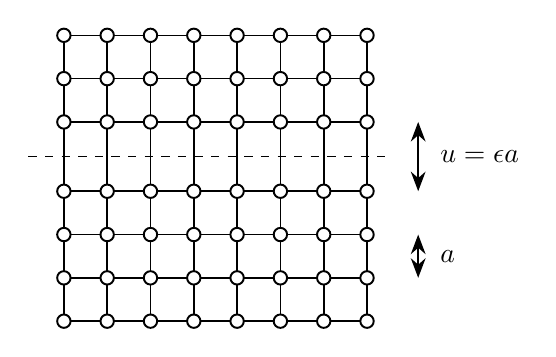
\begin{tikzpicture}[line width=0.8pt,>=Stealth]
\def\sx{0.55}
% row heights: normal 0.55, stretched gap 0.88 between rows 3 and 4
\def\ra{3.30}\def\rb{2.75}\def\rc{2.20}\def\rd{1.32}\def\re{0.77}\def\rf{0.22}\def\rg{-0.33}
% ---- bonds first ----
\foreach \y in {\ra,\rb,\rc,\rd,\re,\rf,\rg}{
  \foreach \c in {0,...,6}{
    \draw[line width=0.6pt] ({\c*\sx},\y) -- ({(\c+1)*\sx},\y);
  }
}
\foreach \ya/\yb in {\ra/\rb,\rb/\rc,\rc/\rd,\rd/\re,\re/\rf,\rf/\rg}{
  \foreach \c in {0,...,7}{
    \draw[line width=0.6pt] ({\c*\sx},\ya) -- ({\c*\sx},\yb);
  }
}
% ---- atoms on top ----
\foreach \y in {\ra,\rb,\rc,\rd,\re,\rf,\rg}{
  \foreach \c in {0,...,7}{
    \draw[fill=white,line width=0.7pt] ({\c*\sx},\y) circle (0.085);
  }
}
% ---- dashed reference line across the stretched interface ----
\draw[dashed,line width=0.55pt] (-0.45,1.76) -- (4.15,1.76);
% ---- right-hand annotations ----
\draw[<->,line width=0.9pt] (4.5,\rc) -- (4.5,\rd);
\node[anchor=west] at (4.65,1.76) {$u=\epsilon a$};
\draw[<->,line width=0.9pt] (4.5,\re) -- (4.5,\rf);
\node[anchor=west] at (4.65,0.495) {$a$};
\end{tikzpicture}
\end{document}
